%%%%%%%%%%%%%%%%%%%%%%%%%%%%%%%%%%%%%%%%%
% Short Sectioned Assignment LaTeX Template Version 1.0 (5/5/12)
% This template has been downloaded from: http://www.LaTeXTemplates.com
% Original author:  Frits Wenneker (http://www.howtotex.com)
% License: CC BY-NC-SA 3.0 (http://creativecommons.org/licenses/by-nc-sa/3.0/)
%%%%%%%%%%%%%%%%%%%%%%%%%%%%%%%%%%%%%%%%%

%----------------------------------------------------------------------------------------
%	PACKAGES AND OTHER DOCUMENT CONFIGURATIONS
%----------------------------------------------------------------------------------------

\documentclass[paper=a4, fontsize=11pt]{scrartcl} % A4 paper and 11pt font size

% ---- Entrada y salida de texto -----

%\usepackage[T1]{fontenc} % Use 8-bit encoding that has 256 glyphs
\usepackage[utf8]{inputenc}
\usepackage[T1]{fontenc}

\usepackage{mathptmx}
\usepackage{fourier}  % Use the Adobe Utopia font for the document - comment this line to return to the LaTeX default

% ---- Idioma --------

\usepackage[spanish, es-tabla]{babel} % Selecciona el español para palabras introducidas automáticamente, p.ej. "septiembre" en la fecha y especifica que se use la palabra Tabla en vez de Cuadro

% ---- Otros paquetes ----

\usepackage{url} % ,href} %para incluir URLs e hipervínculos dentro del texto (aunque hay que instalar href)
\usepackage{amsmath,amsfonts,amsthm} % Math packages
%\usepackage{graphics,graphicx, floatrow} %para incluir imágenes y notas en las imágenes
\usepackage{graphics,graphicx, float} %para incluir imágenes y colocarlas
\graphicspath{ {images/} }
\usepackage{subfig}

\usepackage{algorithm}
\usepackage{algpseudocode}

\usepackage{wrapfig}

% Para hacer tablas comlejas
\usepackage{multirow}
%\usepackage{threeparttable}

%\usepackage{sectsty} % Allows customizing section commands
%\allsectionsfont{\centering \normalfont\scshape} % Make all sections centered, the default font and small caps

\usepackage{fancyhdr} % Custom headers and footers
\pagestyle{fancyplain} % Makes all pages in the document conform to the custom headers and footers
\fancyhead{} % No page header - if you want one, create it in the same way as the footers below
\fancyfoot[L]{} % Empty left footer
\fancyfoot[C]{} % Empty center footer
\fancyfoot[R]{\thepage} % Page numbering for right footer
\renewcommand{\headrulewidth}{0pt} % Remove header underlines
\renewcommand{\footrulewidth}{0pt} % Remove footer underlines
\setlength{\headheight}{13.6pt} % Customize the height of the header

\numberwithin{equation}{section} % Number equations within sections (i.e. 1.1, 1.2, 2.1, 2.2 instead of 1, 2, 3, 4)
\numberwithin{figure}{section} % Number figures within sections (i.e. 1.1, 1.2, 2.1, 2.2 instead of 1, 2, 3, 4)
\numberwithin{table}{section} % Number tables within sections (i.e. 1.1, 1.2, 2.1, 2.2 instead of 1, 2, 3, 4)

\setlength\parindent{0pt} % Removes all indentation from paragraphs - comment this line for an assignment with lots of text

\newcommand{\horrule}[1]{\rule{\linewidth}{#1}} % Create horizontal rule command with 1 argument of height

\usepackage{listings}

\everymath{\displaystyle}
%----------------------------------------------------------------------------------------
%	TÍTULO Y DATOS DEL ALUMNO
%----------------------------------------------------------------------------------------

\title{	
\normalfont \normalsize 
\textsc{\textbf{Periféricos y Dispositivos de Interfaz Humana} \\ Grado en Ingeniería Informática \\ Universidad de Granada} \\ [25pt] % Your university, school and/or department name(s)
\horrule{0.5pt} \\[0.4cm] % Thin top horizontal rule
\huge Reconocimiento Facial  \\ % The assignment title
\horrule{2pt} \\[0.5cm] % Thick bottom horizontal rule
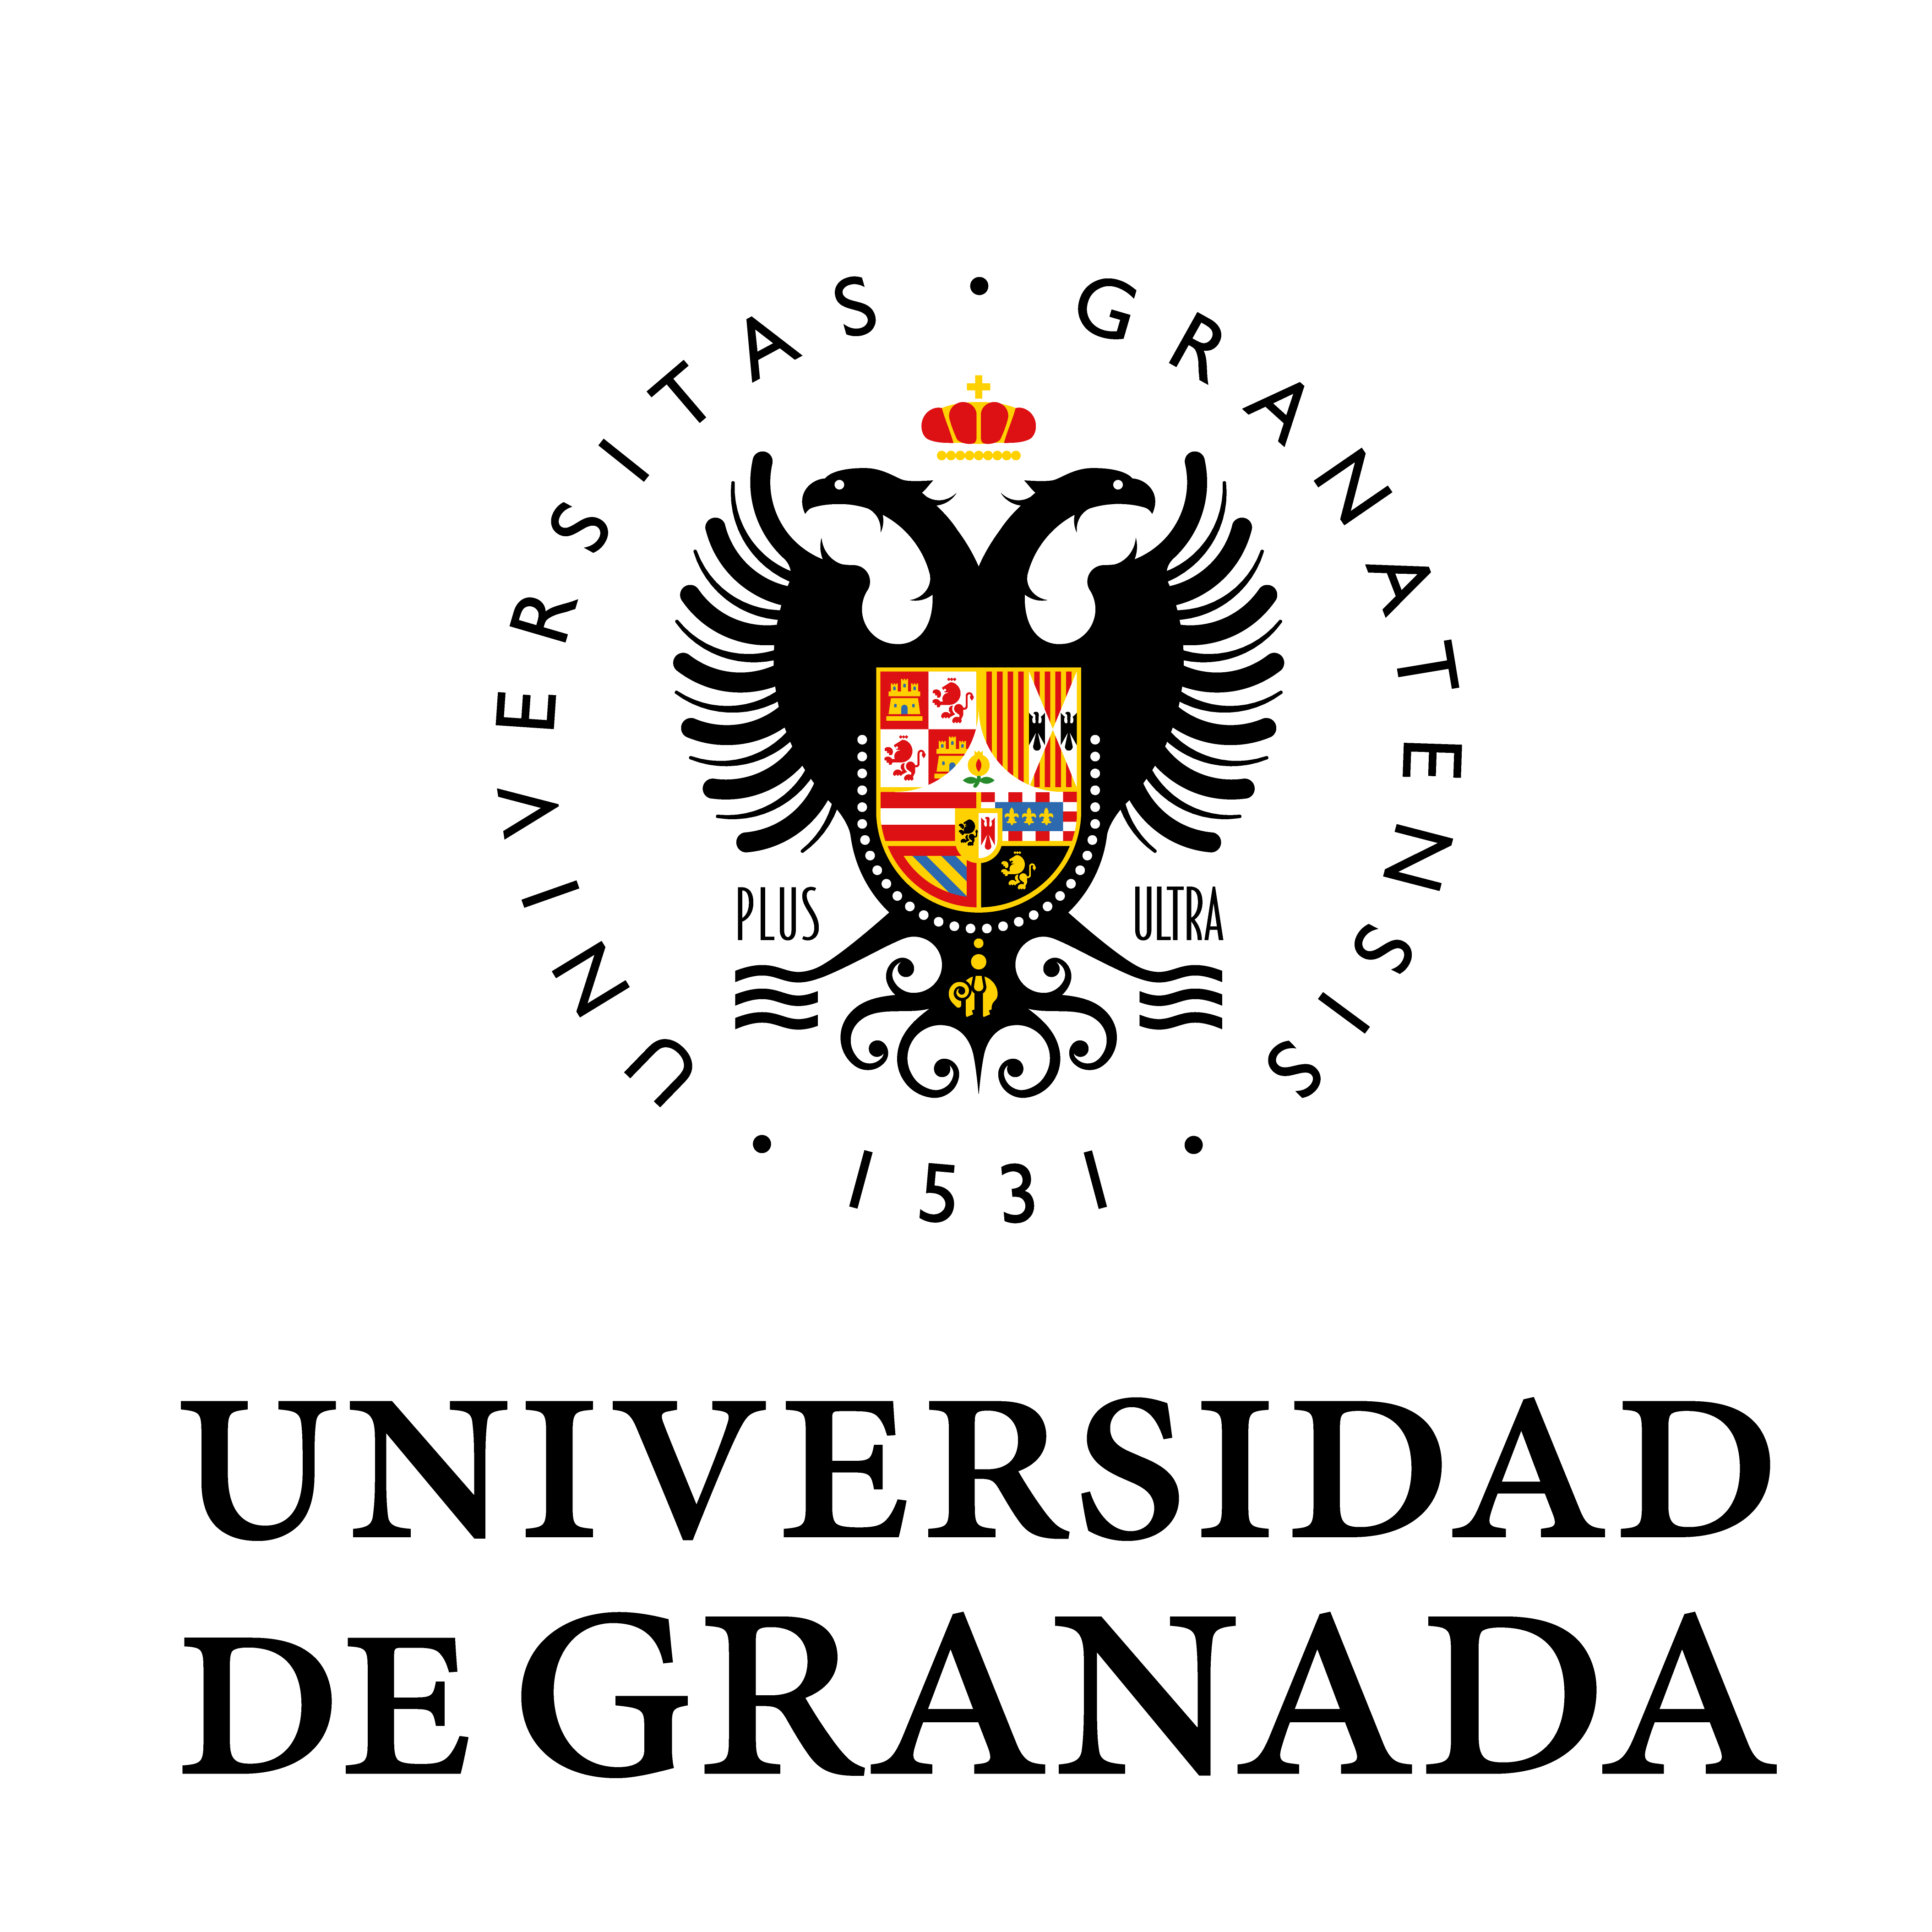
\includegraphics[width=5cm]{logo}\\[8ex]
}




\author{José Luis Molina Aguilar y Sergio España Maldonado} % Nombre y apellidos

\date{\normalsize\today} % Incluye la fecha actual


%----------------------------------------------------------------------------------------
% DOCUMENTO
%----------------------------------------------------------------------------------------

\begin{document}


\maketitle % Muestra el Título
  \begin{large}
    \centering
  \vfill
  
  Curso 2022-2023\\
  Correo : joselu201@correo.ugr.es
  \vfill
  \end{large}
\newpage %inserta un salto de página

\tableofcontents % para generar el índice de contenidos

%\listoftables -----------------------------------------------------------


\newpage



%----------------------------------------------------------------------------------------
%	Cuestión 1
%----------------------------------------------------------------------------------------
\newpage
\section{Descripción}
Vamos a ver dos programas para detectar caras y otro para el reconocimiento de caras,
utilizaremos en ambos Opencv, el primer programa usa algoritmo de cascada para 
detectar caras
el segundo utiliza el modulo de face recognition el cual utiliza deep learning.

\url{https://docs.opencv.org/3.4/db/d28/tutorial_cascade_classifier.html}
\section{ Detección de caras vs Reconocimiento facial}

La detección de caras y el reconocimiento facial son dos términos relacionados 
pero diferentes en el procesamiento de imágenes y la inteligencia artificial.\\

La detección de caras se refiere a la capacidad de detectar la presencia de una 
cara humana en una imagen o video y ubicarla dentro de la imagen. \\

El reconocimiento facial, por otro lado, se refiere a la capacidad de identificar 
una persona en función de sus características faciales. El reconocimiento facial se 
basa en la comparación de las características faciales de una persona con una base 
de datos previamente almacenada de características faciales de personas conocidas.\\

Esta técnica se utiliza en muchas aplicaciones, como la seguridad, el control 
de acceso y la identificación de personas en fotografías o videos.

\section{Modelos de cascada}
Los modelos de cascada son un tipo de algoritmo de detección de objetos que se 
utilizan comúnmente para la detección de rostros en imágenes y videos. 
La detección de cascada se basa en la utilización de una cascada de 
clasificadores que funcionan en serie, donde cada clasificador toma una 
decisión sobre la presencia o ausencia de la característica de interés en una
 determinada región de la imagen.

\begin{figure}[H]
  \centering
  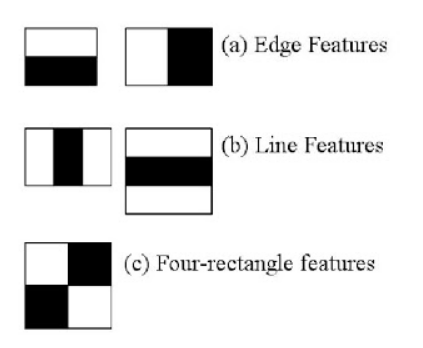
\includegraphics[width=0.5\textwidth]{cascade1}
  \caption{Tipo de Característica}\label{fig:característica}
\end{figure}

Cada característica es un valor único obtenido al restar la suma de píxeles 
debajo del rectángulo blanco de la suma de píxeles debajo del rectángulo negro.

La ventaja de los modelos de cascada es que pueden ser muy rápidos y eficientes 
en la detección de objetos en imágenes y videos, lo que los hace útiles para 
aplicaciones en tiempo real. Sin embargo, también pueden tener limitaciones en 
la detección de objetos en situaciones variables de iluminación, posición y escala



\begin{figure}[H]
  \centering
  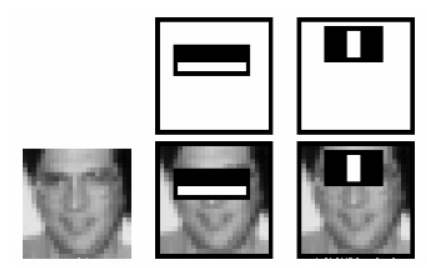
\includegraphics[width=0.5\textwidth]{cascade2}
  \caption{Ejemplo de características}\label{fig:ejemplo_característica}
\end{figure}

La fila superior muestra dos buenas características.\\
La primera característica seleccionada parece centrarse en la propiedad de 
que la región de los ojos suele ser más oscura que la región de la nariz y las mejillas.\\ 
La segunda característica seleccionada se basa en la propiedad de que los ojos son más 
oscuros que el puente de la nariz.\\


Dependiendo de lo que queramos detectar, instanciaremos el clasificador de 
cascada con los diferentes modelos preentrenados que nos ofrece Opencv.

\url{https://github.com/opencv/opencv/tree/4.x/data/haarcascades}

\begin{figure}[H]
  \centering
  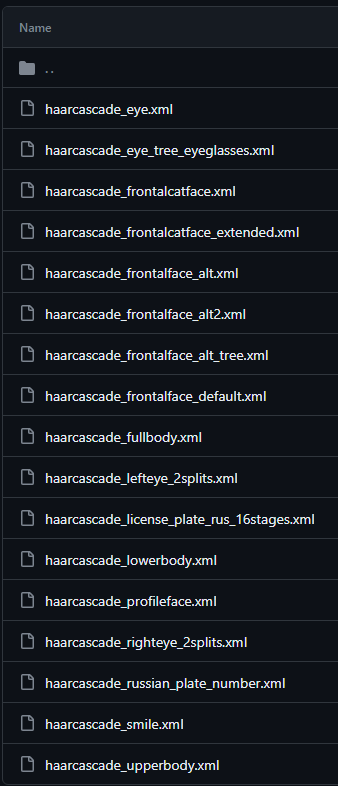
\includegraphics[width=0.5\textwidth]{haarcascade}
  \caption{Diferentes tipo de clasificadores}\label{fig:ejemplo_característica}
\end{figure}



\begin{lstlisting}[language=Python]
  cascade = cv2.CascadeClassifier("haarcascade<ident>.xml")
\end{lstlisting}

y ahora simplemente le pediremos que nos identifique de cada frame de la cámara las caras de la siguiente forma:

\begin{lstlisting}[language=Python]
  res = cascade.detectMultiScale(frame_gris)
\end{lstlisting}

es importante destacar que hay que convertir el frame en rgb a escala de grises,
esto nos devuelve las coordenadas de la parte superior izquierda de la cara y su 
ancho y largo




\section{Python face\_recognition}

Ahora utilizaremos un modulo de Python llamado face\_recognition
\url{https://pypi.org/project/face-recognition/}
necesitaremos tener un par de cosas instaladas antes, como cmake, dlib y visual studio.

face-recognition es una herramienta de software libre y de código abierto
que se utiliza para el reconocimiento facial y la detección de características en imágenes.\\

Proporciona una interfaz de programación de aplicaciones (API) fácil de usar
para realizar tareas de reconocimiento facial, incluyendo la detección de caras,
la extracción de características faciales y la comparación de caras para
la identificación de individuos.\\

Una vez que se han detectado las caras, la biblioteca face-recognition
utiliza un algoritmo de extracción de características faciales basado en 
"dlib" para obtener un vector de características únicas para cada cara detectada.\\
Estas características incluyen la forma de la cara, las distancias entre los ojos,
la nariz y la boca, y otros detalles únicos que se utilizan para identificar a una persona.\\

Es importante destacar que Opencv utiliza los colores bgr (blue, green, red)
en vez de rgb, por esto mismo cada vez que leamos una imagen tendremos que modificar 
su representación ya que face\_recognition si que utiliza rgb.

Utilizaremos la función face\_location para localizar las caras de la imagen
\begin{lstlisting}[language=Python]
  import face_recognition as face
  locs = face.face_locations(framergb)
\end{lstlisting}

una vez que tenemos esto para poder diferenciar a las personas tendremos que buscar sus
característica faciales, eso lo haremos de la siguiente forma. 

\begin{lstlisting}[language=Python]
  lands = face.face_landmarks(framergb)
\end{lstlisting}

Ahora tenemos un diccionario en el cual representamos la facción de la cara con su valor.
Ahora que tenemos esto, para comparar las caras y determinar la identidad utilizaremos 
face encodings que devuelve un vector de característica.
Estos vectores de características se pueden utilizar para identificar y comparar caras.

\begin{lstlisting}[language=Python]
  cod_micara = face.face_encodings(framergb,locs,model='small')[0]
\end{lstlisting}

Le pasamos la imagen y las posiciones donde hemos localizado las caras, tenemos un tercer parámetro
que indica el modelo este se utiliza para especificar el modelo que se utilizará para la detección de caras.
Puede ser 'small' para un modelo más rápido pero menos preciso, o 'large' para un modelo más preciso pero más lento.

Ahora simplemente repetiremos estos pasos con cada imagen de la cámara para poder comparar la imagen de referencia
con las de la cámara

\begin{lstlisting}[language=Python]
  face.compare_faces(cod_micara, cara_cam)
\end{lstlisting}


\end{document}
